% Influence of the radius of sight of an agent

\noi In this test series, the constant variable INFLUENCESPHERE, which determines the radius of the semi-circle in which the agent considers other agents around him, was varied. First of all, the dependency between the influence sphere's radius and the total distance walked by all agents had to be evaluated.\\

\begin{figure}[h!]
	\centering
		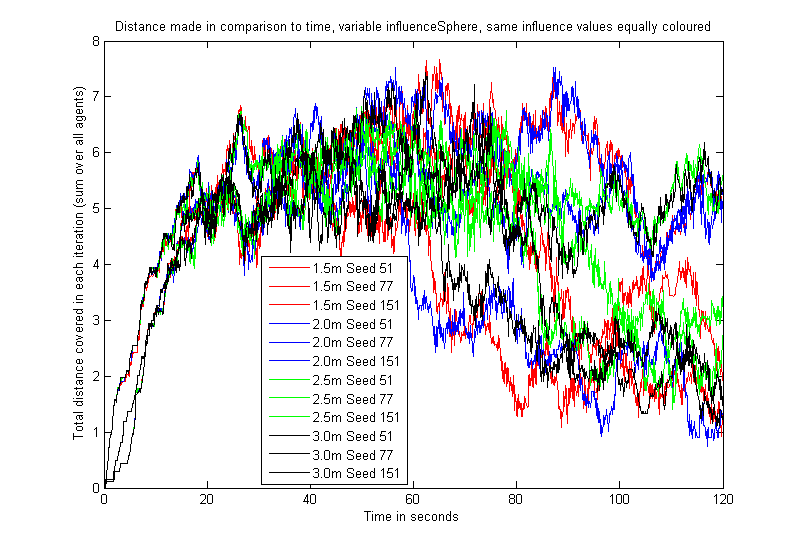
\includegraphics[width=0.80\textwidth]{pictures/ATotalDistanceInfluencesColoured.png}
	\caption{This plot shows the total distance covered by all agents in the system for different influence sphere radii and seeds in dependence of the simulation time. This distance decreases rapidly when a jam starts. To show the total distance's dependence on the influence sphere radius, each seed to a certain radius was coloured equally. One can see here that there is no clear dependence of the radii to the total distance as for every radius except 1.5 m there are seeds that work and seeds that don't, which means they had jams.}
	\label{fig:InfluencesColoured}
\end{figure}

\noi As shown in figure \ref{fig:InfluencesColoured}, neither dependencies nor tendencies can be seen clearly, as for every tested radius of influence, some seeds worked well where other simulations for the same seed jammed.

\begin{figure}[h!]
	\centering
		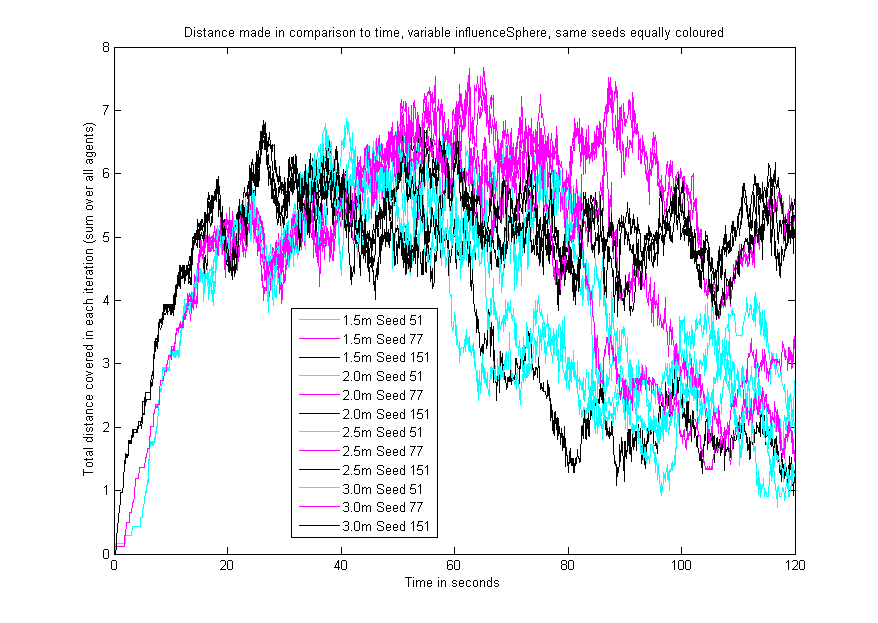
\includegraphics[width=0.80\textwidth]{pictures/ATotalDistanceSeedsColoured.png}
	\caption{This plot shows the total distance covered by all agents in the system for different influence sphere radii and seeds in dependence of the simulation time. This distance decreases rapidly when a jam starts. To show the total distance's dependence on the seed, each radius to a certain seed was coloured equally. One can see here that whether a simulation jams or not seems to depend on the seed, as the seed 51 simulations all jammed independent of the radius, and for the other two seeds, there was only one radius that was different.}
	\label{fig:SeedsColoured}
\end{figure}

\noi Next, there maybe is a dependence between the success of a simulation and the seed which would explain why no clear tendencies for the radii was observed in figure \ref{fig:InfluencesColoured}. So, in figure \ref{fig:SeedsColoured}, the same seeds were coloured equally, which showed much more of a tendency: A seed seems to have the property that it will most likely jam or not: Seed 51 caused jams for every radius, whereas seed 77 and seed 151 produced a similar result except for outliers.

\begin{figure}[h!]
	\centering
		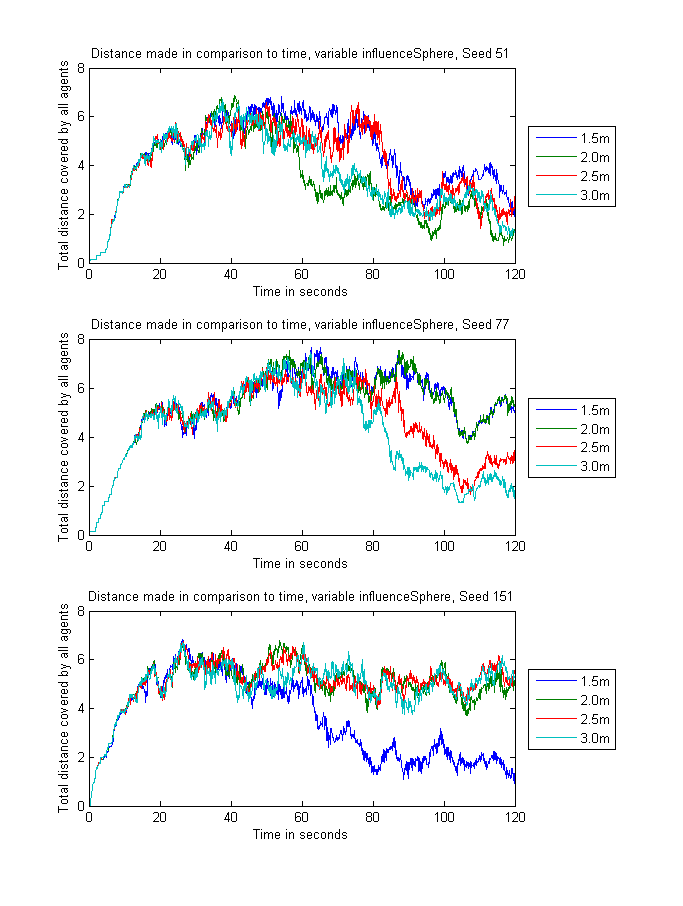
\includegraphics[width=0.75\textwidth]{pictures/ADistancesPerSeeds.png}
	\caption{This plot shows the total distance covered by all agents in the system for different influence sphere radii and seeds in dependence of the simulation time. This distance decreases rapidly when a jam starts. To investigate the radius' dependence on the total distance, the total plot was split up into three parts, each containing all simulations for one seed. One can see here that in seed 51, every simulation jammed independently of the radius. In seed 77, the larger radii jammed, on the other hand only the small radius crashed in seed 151.}
	\label{fig:SeedsOverview}
\end{figure}

\noi To investigate this further, the plot was now split up into 3 subplots with one for each seed as given in figure \ref{fig:SeedsOverview}. Again, this seems to show some dependency as assumed in figure \ref{fig:SeedsColoured}, but this could also be coincidence.\\
Here, no dependency can be seen because with seed 51, every single simulation will cause jams. Seed 151 shows what one could expect to see: For a small influence sphere radius, a jam pops up. But seed 77 shows the exact opposite of this as here, the larger influence radii caused jams. So neither dependence nor tendency between influence sphere radius and total distance walked can be observed.\\

\noi These results are not really surprising as we weighted short distance interactions quadratically, therefore the inclusion of more influences with a big distance should not have a big effect. This could change if the weighting would not be quadratic but maybe linear, but then the agents should bump into each other much more frequently.\\

%Discussion -> Discussion (Y)
As already seen in chapter \textbf{hier verweis zur resultate-section von dieser serie einf�gen}, neither dependence nor tendency between influence sphere radius and total distance walked can be observed because there were opposing trends. Seed 151 showed what we expected to see: For a small influence radius, a jam popped up where for larger radii it didn't. On the other hand, seed 77 showed the exact opposite: only the large radii caused jams.\\
This leads us to think that coicidence played a main role here and shows us another thing: In our formulas weighing the influence of other agents on a specific agents, the weights are too big for very close agents in comparison to agents in a larger distance. This explains why larger radii didn't show the expected results: the additional influence of those agents was too little to matter. The assumption that out weighing function is not perfect can also be observed in any simulation: The agents walk straight forwards to each other for a long time and avoid each other only when they are very close to each other and not from a few meters ahead.
